Pour cette gamme de simulation, nous avons choisi de revenir sur un jeu de conditions proche de notre première idée. Nous allons plonger une sphère de Hénon dans un bain homogène remplissant une boîte.
La première chose à faire est de stabiliser le cube. Mais présentons d'abord le système d'unité utilisé ici.

\subsection{Système d'unité}
	\label{simu::sec::unit}
	Nous nous plaçons dans le système décrit dans \cite{fuji1983}. C'est à dire:
	\begin{itemize}
		\item $\tilde{M_h} = 1$
		\item $\tilde{R_0} = 2$
		\item $\tilde{G} = 1$
	\end{itemize}

	Le changement de variable a effectué pour passer des unités physiques à celle de l'article est le suivant:
	\begin{align}
		\begin{cases}
			\tilde{m} = \frac{m}{M_t} \\
			\\
			\tilde{r} = \frac{r}{R_0} \\
			\\
			\tilde{v} = \frac{v}{\sqrt{\frac{GM_t}{R_0}}}
		\end{cases}
	\end{align}
	Point intéressant, le temps dynamique devient:
	\begin{align}
		T_d = \pi \sqrt{\frac{R_0^3}{2GM}} = 2\pi
	\end{align}

\subsection{Stabilité du cube}
	\begin{wrapfigure}{l}{0.20\textwidth}
		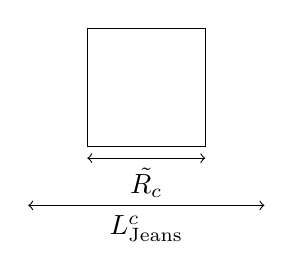
\begin{tikzpicture}[scale=1.5]
			\draw (0, 0) -- (1, 0) -- (1, 1) -- (0, 1) -- (0, 0);
			\draw[<->] (0, -0.1) -- (1, -0.1);
			\draw (0.5, -0.1) node[below] {$\tilde{R_c}$};
			\draw[<->] (-0.5, -0.5) -- (1.5, -0.5);
			\draw (0.5, -0.5) node[below] {$L_\mathrm{Jeans}^c$};
		\end{tikzpicture}
	\end{wrapfigure}
	Vouloir faire une simulation avec un cube interagissant, c'est bien beau, mais un tel objet risque de s'effondrer plutôt vite. Il va nous falloir une condition pour pouvoir le stabiliser.
	Une sphère homogène est stable si sa taille est inférieur à sa longueur de Jeans. Notre critère est donc le suivant:
	\begin{align}
		R_c &\le L_\mathrm{Jeans}^c = \dfrac{\sigma_c^2}{\sqrt{G\rho_c}} \\
		R_c^2 &\leq \dfrac{\sigma_c^2}{G\rho_c} \notag \\
		R_c^2 &\leq \dfrac{\sigma_c^2 R_c^3}{GM_c} \notag \\
		\intertext{Soit $N_c$ le nombre de particules du cube:} \\
		1 &\leq \dfrac{\sigma_c^2R_c}{GN_c m_c} \notag
	\end{align}
	Nous imposons aux particules du cube d'avoir la même masse que celle du Hénon, soit:
	\begin{align*}
		m_c = m_h = m = \dfrac{M_h}{N_h}
	\end{align*}
	où $N_h$ est le nombre de particules du Hénon. Notre critère devient:
	\begin{align}
		1 &\leq \dfrac{\sigma_c^2R_cN_h}{GN_c M_h} \notag \\
		GM_h\dfrac{1}{\sigma_c^2}\dfrac{N_c}{N_h} &\leq R_c \notag
	\end{align}
	en oubliant pas que: $G=1$ et $M_h=1$.
	\begin{align}
		\dfrac{1}{\sigma_c^2} \dfrac{N_c}{N_h} &\leq R_c \label{simu::eq::idee4_jeans}
	\end{align}
	

\subsection{Conditions de la simulation}
	Comme nous cherchons à vérifier notre modèle, nous devons placer le bain à une température
	inférieur à celle que la sphère de Hénon atteint une fois à l'équilibre. Soit $\sigma_h^f$ la
	dispersion de vitesse de la sphère après effondrement, on doit avoir:
	\begin{align}
		\sigma_c &< \sigma_h^f \label{simu::eq::idee4_sig}
	\end{align}

	En parallèle, il serait bon d'éviter que le bain détruise la sphère de Hénon. Il faudrait
	donc avoir:
	\begin{align}
		\rho^f\(R\) \geq \rho_c \label{simu::eq::idee4_dens}
	\end{align}
	où $\rho^f\(R\)$ représente la densité au bord de la sphère, une fois l'équilibre
	atteint.

\subsection{Critères de sélections des paramètres}
	En combinant les équations \ref{simu::eq::idee4_dens}, \ref{simu::eq::idee4_sig} et
	\ref{simu::eq::idee4_jeans}, nous obtenons l'ensemble d'équations suivant:
	\begin{align}
		\begin{cases}
			\dfrac{1}{\sigma_c^2} \dfrac{N_c}{N_h} \leq R_c \\
			\\
			\sigma_c < \sigma_h^f
		\end{cases}
	\end{align}
	%avec $R_h$ le rayon de la sphère une fois l'équilibre atteint, sans le bain.

\subsection{Jeux des paramètres}
	Pour vérifier l'influence du bain, nous devrons jouer sur sa température (sa dispersion de vitesse).
	Mais, nous souhaitons conserver les autres paramètres les moins inchangées possible. Par exemple,
	tel que la simulation est construite, un certains nombres de particules $n_c$ sont directement
	incluse dans le Hénon qui se retrouve alors avec $N_h + n_c$ particules et donc une masse de $M_h + n_c m$.
	De ce fait, pour avoir les simulations les plus similaires possible, nous devons conserver la densité moyenne
	du cube $\rho_c$ constante afin de conserver au mieux $n_c$.

	Voyons comment se comporte notre système:
	\begin{align}
		\rho_c = \dfrac{M_c}{R_c^3} = \dfrac{mN_c}{R_c^3}
	\end{align}
	Nous faisons évoluer notre dispersion de vitesse tel que:
	\begin{align*}
		\sigma_c' = k \sigma_c
	\end{align*}
	en conservant:
	\begin{align}
		\rho_c' = \rho_c \label{simu::eq::idee4_cubedens}
	\end{align}
	Le nouveau rayon s'écrit:
	\begin{align}
		R_c' &= \dfrac{1}{\sigma_c'^2}\dfrac{N_c'}{N_h} = \dfrac{1}{k^2\sigma_c^2}\dfrac{N_c'}{N_h} \notag \\
		\intertext{En utilisant \ref{simu::eq::idee4_cubedens}:}
		\rho_c' &= \rho_c \notag \\
		\dfrac{m N_c}{\(\dfrac{1}{k²\sigma_c²}\dfrac{N_c'}{N_h}\)^3} &= \dfrac{m N_c}{\(\dfrac{1}{\sigma_c²}\dfrac{N_c}{N_h}\)^3} \notag \\
		\dfrac{1}{\dfrac{1}{k^6}N_c'^2} &= \dfrac{1}{N_c^2} \notag \\
		N_c' &= k^3 N_c
	\end{align}
	Ainsi, en augmentant d'un facteur $k$ la dispersion de vitesse, il faut augmenter d'un facteur $k^3$ le nombre de particules dans le cube.

\subsection{Test de stabilité du cube dans ces conditions}
	\begin{figure}
		\begin{center}
			\includegraphics[width=\textwidth]{graphe/dc.png}
			\caption{Carte de l'objet à $t=0$}
			\label{simu::graphe::dccarte0}
		\end{center}
	\end{figure}
	\begin{figure}
		\begin{center}
			\includegraphics[width=\textwidth]{graphe/dc500.png}
			\caption{Carte de l'objet à $t=50$}
			\label{simu::graphe::dccarte50}
		\end{center}
	\end{figure}
	\begin{figure}
			\begin{minipage}[b]{0.40\linewidth}
				\centering \includegraphics[width=\textwidth]{graphe/test_simu_temp.pdf}
				\caption{Température moyenne de l'objet}
				\label{simu::graphe::temp}
			\end{minipage}\hfill
			\begin{minipage}[b]{0.48\linewidth}
				\centering \includegraphics[width=\textwidth]{graphe/test_simu.pdf}
				\caption{Viriel de l'objet}
				\label{simu::graphe::viriel}
			\end{minipage}
	\end{figure}

\subsection{Évolution d'une sphère de Hénon isolée}
	\subsubsection{Évolution dans le vide}
		Des simulations sur l'évolution d'une sphère de Hénon dans le vide on été faîte avec le même
		jeux de paramètres. Ces simulations serviront de référence pour celle avec bain. Toutes ont
		été faîtes jusqu'au temps $t = 50$ dans les unités indiqués section~\ref{simu::sec::unit}.

		\begin{figure}
			\begin{center}
				\includegraphics[width=\textwidth]{graphe/All_parameters.pdf}
				\caption{Évolution dans le temps des paramètres}
				\label{simu::graphe::Parameter}
			\end{center}
		\end{figure}

	\subsection{Effet du nombre de particule}
		Les simulations mentionnées dans le paragraphe précèdent ont été faîtes avec 300 000 et 1 000 000
		de particules. Le graphique~\ref{simu::graphe::densitecomp} compare les profiles de densité volumiques de masse
		à la fin de chacune des simulations.

		\begin{figure}
			\begin{center}
				\includegraphics[width=\textwidth]{graphe/comparison_between_310part.pdf}
				\caption{Comparaison de l'état final entre une simulation de 300 000 particules et une de 1 000 000 de particules.}
				\label{simu::graphe::densitecomp}
			\end{center}
		\end{figure}

